\begin{figure}[H]
\centering
  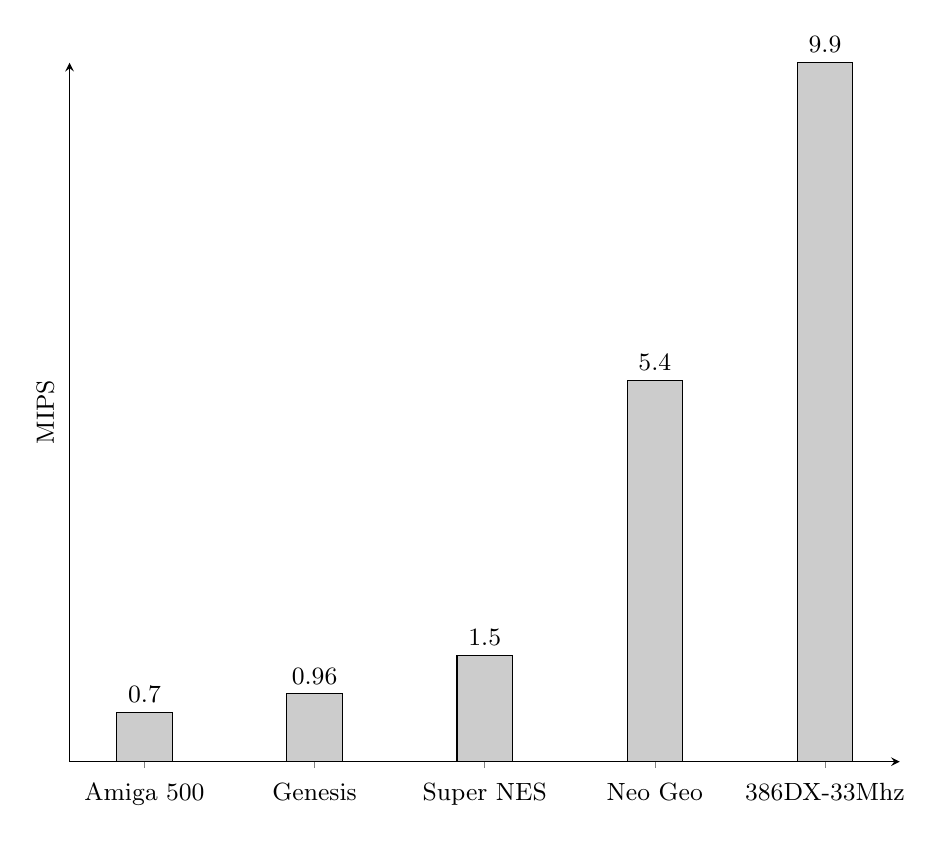
\begin{tikzpicture}[font=\small]
    \begin{axis}[
      width=\textwidth,
      %height=0.6\textwidth,
      ybar=6pt,
      bar width=20pt,
      ylabel={MIPS},
      ymin=0,
      ytick=\empty,
      xtick=data,
      axis x line=bottom,
      axis y line=left,
      enlarge x limits=0.11,
      symbolic x coords={Amiga 500, Genesis, Super NES, Neo Geo,386DX-33Mhz},
      xticklabel style={anchor=base,yshift=-\baselineskip},
      nodes near coords={\pgfmathprintnumber\pgfplotspointmeta}
    ]
      \addplot[fill=black!20,draw=black] coordinates {
        (Amiga 500,0.7)
        (Genesis,0.96)
        (Super NES,1.5)
        (Neo Geo,5.4)
        (386DX-33Mhz,9.9)
      };
    \end{axis}
   \end{tikzpicture}
   \caption{Game Console Vs PC: CPU comparison with MIPS\protect\footnotemark.}
   \label{fig:ems_xms_layout}
 \end{figure}
 \footnotetext{Million Instructions Per Second.}
